% !TEX TS-program = XeLaTeX
\documentclass{CSICC2016}

% تقریبا تمامی بسته‌های مورد نیاز برای یک مقاله در استایل فراخوانی شده است. اما در هر صورت در صورتی‌که می‌خواهید بسته‌ای را فراخوانی کنید به صورت زیر عمل کنید. مثلا ما در کد زیر دوبسته glossaries و tikz را فراخوانی کرده‌ایم.
%\makeatletter
%\bidi@BeforePackage{xepersian}{
%\RequirePackage{tikz}
%\RequirePackage{glossaries}
%}
%\makeatother

\usepackage{
                graphicx, setspace, fontspec, caption,
                subcaption, float,
                lscape, pdflscape, indentfirst,
                multirow, mathtools, currfile,
				url, chngpage, flexisym, amsfonts, chngpage
            }

\usepackage[justification=centering]{caption}

\renewcommand{\ }{\hspace{0em}}
\newcommand{\مق}{\lr}
\renewcommand{\یا}{یادگیری\ ارجحیت }
\newcommand{\یم}{یادگیری\ ماشین }
\renewcommand{\تر}{تابع رتبه\ بند }
\newcommand{\ار}{ارجحیت }
\renewcommand{\|}[1][.3em]{\hspace{#1}|\hspace{#1}}
\renewcommand{\,}[1][.3em]{,\hspace{#1}}

\newcommand{\outOne}{N_{\succ}}
\newcommand{\outTwo}{N_{\prec}}
\newcommand{\outOneXY}{\outOne([x,y])}
\newcommand{\outTwoXY}{\outTwo([x,y])}
\newcommand{\xy}{x \succ y}
\newcommand{\yx}{y \succ x}

\graphicspath{ {images/} }

% عنوان مقاله را در این قسمت وارد کنید. 
\title{
یادگیری ارجحیت با استفاده از شبکه\ های عصبی مصنوعی
}
\date{}
% اسامی نویسندگان و همچنین اطلاعات مربوط به آن‌ها را در این قسمت وارد کنید. 
\author[1]{داریوش حسن\ پور آده}
\affil[1]{
دانشگاه صنعتی اصفهان، دانشکده مهندسی برق و کامپیوتر\\
شماره دانشجویی: ۹۳۰۸۱۶۴
}

\begin{document}
\maketitle
\begin{abstract}
\یا یکی از زیررشته\ های \یم می\ باشد که هدف اصلی\ اش یادگیری ارجحیت\ های قابل پیش\ بینی از روی اطلاعات ارجحیت می\ باشد. از نقطه\ نظر یادگیری باناظر \یا روی یک دسته از عناصر که نسبت به یک دسته از برچسب\ ها یا عناصر ارجحیت بیشتری دارند آموزش داده می\ شوند که بتواند در نهایت مدل ارجحیت عناصر دیده نشده را پیش\ بینی کند. در این گزارش با تکیه بر مطالب مقاله\ ی اصلی به معرفی یک روش یادگیری جهت یادگیری رتبه\ بندی\زیرنویس{\مق{Rank}} می\ پردازیم که توسط شبکه\ ای به نام \مق{CmpNN} به رتبه\ بندی میان اشیا می\ پردازد. شبکه\ ی معرفی شده دارای معماری خاصی بوده و الگوریتمی که معرفی شده به نحو خاصی آموزش داده می\ شود تا بهترین توصیف آموزشی متناسب با وزن\ های شبکه و داده\ های آموزشی را مشاهده کند. همچنین در کنار شرح مقاله\ ی اصلی به مروری بر دیگر کارهای انجام شده در زمینه\ ی \یا با شبکه\ های عصبی مصنوعی خواهیم پرداخت.
\end{abstract}
\begin{keywords}
یادگیری ارجحیت، شبکه\ های عصبی مصنوعی، شبکه\ ی ارجحیت، یادگیری انتخابی، ‌طبقه\ بندی
\end{keywords}

\قسمت{مقدمه}

یادگیری ارجحیت\زیرنویس{\lr{Preference Learning}} یکی از شاخه\ های یادگیری\ ماشین\زیرنویس{\lr{Machnine Learning}} می\ باشد که در سال\ های اخیر توجه زیادی را به سمت خود جلب کرده است. وظیفه\ ی اصلی یادگیری\ ارجحیت، \emph{یادگیری رتبه\ بندی کردن} عناصر می\ باشد. که با توجه به نوع اطلاعات آموزشی نوع ارجحیت و همچنین نوع رتبه\ بندی می\ تواند تغییر کند. در حالت کلی \یا به استنتاج کردن ارتباطات بین اعضای یک دسته و نگاشت این ارتباطات به مدلی که بتواند ارجحیت نسبی موجود بین اعضای این دسته بخوبی پیش\ بینی کند.\بند
اگر بخواهیم تعریف دقیقی برای \یا ارائه دهیم می\ توانیم بگوییم که \یا به وظیفه\ ی یادگیری پیش\ بینی کردن رابطه\ ی ترتیب\زیرنویس{\lr{Order}} در مجموعه\ ای از اشیا گفت\
\cite{PL:PL_PEDIA}.
\یا از داده\ های اطلاعات ارجحیت\زیرنویس{\lr{Preference Information}} برای اهداف یادگیری خود استفاده می\ کند که این اطلاعات ارجحیت نقش مهمی در تصمیم\ گیری\ های خودکار در زمینه\ های متعددی مانند تئوری تصمیم\ گیری\ های کیفی\
\زیرنویس{\lr{Qualitative decision theory}}،
استدلال غیریکنواخت\
\زیرنویس{\lr{Non-monotonic reasoning}}،
ارضای محدودیت\زیرنویس{\lr{Constraint satisfaction}} و طرح\ ریزی\زیرنویس{\lr{Planning}} و \ldots\hspace{.01em}
 کاربردهای فراوانی دارد. در مرحله\ ی آموزش، الگوریتم\ های \یا به داده\ های ترتیب رتبه\ بندی\زیرنویس{\lr{Ranking Order}} (نیمه)شناخته شده عناصر دسترسی دارند. بسته به مدل و نوع مساله الگوریتم\ های \یا می\ توانند به ۳ دسته\ ی رتبه\ بندی اشیا\زیرنویس{\lr{Object Ranking}}، رتبه\ بندی برچسب\ ها\زیرنویس{\lr{Label Ranking}} و رتبه\ بندی نمونه\ ها\زیرنویس{\lr{Instance Ranking}} تقسیم\ بندی کرد.
\بند در این نوشتار ابتدا مقدمه\ ای بر مفاهیم بنیادی مطرح در \یا آورده شده است و بعد از مروری خلاصه بر تعدادی از کارهای انجام شده در این زمینه، با تمرکز بر مقاله اصلی \یا با استفاده از \مق{ANN} را ارائه خواهیم داد.

\قسمت{\یا}
برای اینکه بتوانیم \emph{\یا با استفاده از شبکه\ های عصبی مصنوعی} را ارائه دهیم نیاز هست که در این قسمت به معرفی خلاصه\ ای از مفاهیم اولیه و بنیادی زمینه\ ی \یا بپردازیم.

\زیرقسمت{نمادگذاری}
طبق هر شاخه\ ی علمی دیگر به یک سری نماد برای پایه\ گذاری \یا نیاز داریم که در این قسمت به معرفی آن\ ها می\ پردازیم.

\begin{definition}[ارجحیت ضعیف]\label{DEF:WEAK_PREF}
یک ارجحیت ضعیف با نماد $\succeq$ بروی مجموعه\ ای مانند $\mathcal{A}$ یک رابطه\ ی بازتابی و تعددی می\ باشد.
\end{definition}

\begin{definition}[ارجحیت اکید]\label{DEF:STRICT_PREF}
$a \succ b \leftrightarrow (a \succeq b) \wedge (b \not\succeq a)$
\end{definition}

در راستای معناشناسی \یا تعاریف
\ref{DEF:WEAK_PREF} و \ref{DEF:STRICT_PREF}
می\ توان آن\ ها را به صورت جدول
\ref{TAB:NOTATIONS_SEMANTIC}
تعبیر کرد.
\vspace{1.5em}
\begin{table}[H]
    \centering
    \begin{tabular}{c|c}
        \textit{نماد} & \textit{تعبیر} \\\hline\rule{0pt}{1.6em}
        $a \succeq b$ & "جایگزین $a$ حداقل به اندازه\ ی جایگزین $b$ ترجیح داده می\ شود." \\\rule{0pt}{1.6em}
        $a \succ b$ & "جایگزین $a$ بیشتر از جایگزین $b$ ترجیح داده می\ شود."\\
    \end{tabular}
    \caption{تعبیر نمادهای روابط ارجحیت}\label{TAB:NOTATIONS_SEMANTIC}
\end{table}
\vspace{.5em}
\begin{definition}[ترتیب\ اکید کلی\زیرنویس{\lr{Total Strict Order}} -- رتبه\ بندی\زیرنویس{\lr{Order}}]\label{DEF:TOT_STRICT_ORDER}
اگر $\mathcal{A}$ یک مجموعه\ ای از اشیا / جایگزین\ ها\زیرنویس{\lr{Alternatives}} $\{a_1\,\ldots\,a_m\}$ باشد، یک رتبه\ بندی از $\mathcal{A}$ یک جایگشتی همانند $\tau$ از مجموعه\ ی $\{1\,\ldots\,m\}$ می\ باشد بگونه\ ای که $a_i \succ a_j \leftrightarrow \tau(i) < \tau(j)$.
\end{definition}
در تعریف
\ref{DEF:TOT_STRICT_ORDER}
مقدار
$m$
تعداد اشیا/جایگزین\ ها و $a_i$ها همان اشیا/جایگزین\ ها می\ باشند،‌ که از این به بعد به مجموعه\ ی اشیا یا جایگزین\ ها، فقط \emph{جایگزین} گفته خواهد شد. تعریف
\ref{DEF:TOT_STRICT_ORDER}
در واقع فرمت\زیرنویس{\lr{Format}} خروجی کلی الگوریتم\ های \یا را ارائه می\ دهد،‌ به گونه\ ای که خروجی ارجحیت ورودی\ ها یک جایگشتی اندیسی\زیرنویس{\lr{Index Permutation}} ترتیب\ اکید ارجحیت\ های ورودی\ ها می\ باشد بگونه\ ای که \textbf{اندیس} آن جایگزینی که \textbf{دارای ارجحیت بیشتری} نسبت به دیگری است، در مجموعه\ ی $\tau$ \textbf{مقدم\ تر} از دیگری می\ آید.\بند
طبق آنچه که در تعریف
\ref{DEF:TOT_STRICT_ORDER}
آمده، واضح است که الگوریتم\ های \یا درواقع یک جستجوکننده در فضای جایگشتی مجموعه $\tau$ می\ باشد؛ فضای جایگشت\ های $\tau$ را با $\mathcal{S}_m$ نمایش می\ دهند.

\زیرقسمت{انواع الگوریتم\ های رتبه\ بندی}
\label{SUBSEC:TYPES_OF_RANKING_PROBLEMES}
الگوریتم\ های رتبه\ بندی از نظر نوع وظیفه\ ای که به عهده دارند به ۳ تیپ تقسیم\ بندی می\ شوند که عبارتند از رتبه\ بندی برچسب\ ها، رتبه\ بندی اشیا و رتبه\ بندی نمونه\ ها؛ که در این قسمت شرح مختصری از این ۳ تیپ الگوریتم ارائه خواهیم داد\
\cite{PL:PL_PEDIA}.
\زیرزیرقسمت{رتبه\ بندی برچسب\ ها}
در این رتبه\ بندی هدف این است که به ازای یک نمونه برچسب\ ها را براساس ارجحیت مرتب کند. شماتیک ورودی\ ها و خروجی\ ها این نوع الگوریتم در شکل
\ref{FIG:LABEL_RANKING_SCHEMA}
آمده است.
\begin{figure}[H]
    \centering
    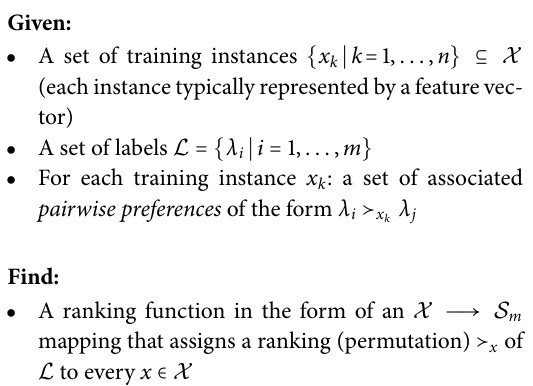
\includegraphics[width=.4\textwidth]{label-ranking}
    \caption{شماتیک کلی الگوریتم\ های رتبه\ بندی برچسب\ ها}\label{FIG:LABEL_RANKING_SCHEMA}
\end{figure}
همانطور که در شکل
\ref{FIG:LABEL_RANKING_SCHEMA}
آمده است الگوریتم\ های رتبه\ بندی برچسب\ ها تعدادی نمونه\ ی آموزشی می\ گیرد که این نمونه\ های آموزشی معمولا به صورت بردار ویژگی\ ها نمایش داده می\ شود. سپس یک سری برچسب و همچنین به ازای هرکدام از نمونه\ ها یک مجموعه\ ی دوبه\ دو مرتب که ارجحیت برچسب\ ها برای هرکدام از نمونه\ ها مشخص شده است را به عنوان ورودی به الگوریتم داده می\ شود.الگوریتم\ های متعلق به رتبه\ بندی برچسب\ ها باید به عنوان خروجی یک \تر است که بتواند به ازای یک شی جایگشت\ های برچسب\ های متعلق به آن شی را با توجه به ارجحیتی که دارند برگرداند.

\زیرزیرقسمت{رتبه\ بندی اشیا}
\label{SEC:OBJECT_RANKING}
در این رتبه\ بندی هدف این است که یک دسته از اشیا را برحسب ارجحیتی که نسبت به هم دارند، را مرتب\ سازی کنیم. که شماتیک ورودی\ ها و خروجی\ ها این نوع الگوریتم در شکل
\ref{FIG:OBJECT_RANKING_SCHEMA}
آمده است.
\begin{figure}[H]
    \centering
    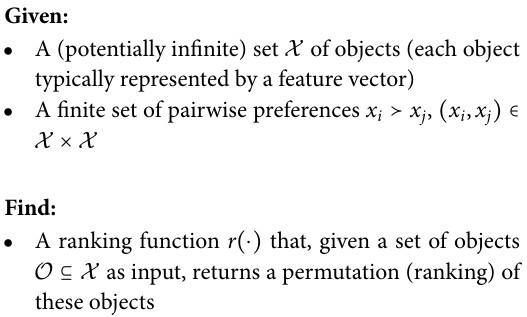
\includegraphics[width=.4\textwidth]{object-ranking}
    \caption{شماتیک کلی الگوریتم\ های رتبه\ بندی اشیا}\label{FIG:OBJECT_RANKING_SCHEMA}
\end{figure}
در شماتیکی که در شکل
\ref{FIG:OBJECT_RANKING_SCHEMA}
آمده است می\ بینیم که همانند رتبه\ بندی برچسب\ ها یک دسته از اشیا را به عنوان ورودی می\ گیرد. سپس یک دسته\ ی (تکه\ ای)مرتب از ارجحیت\ های نسبی این اشیا را نیز به عنوان ورودی به الگوریتم می\ دهیم و نهایت الگوریتم باید یک \تر را بیابد که بتواند ارجحیت\ های هر زیرمجموعه از مجموعه\ ی جهانی اشیا را در قالب یک جایگشتی از اشیا ورودی به عنوان خروجی برگرداند.\بند
توجه شود که مجموعه\ ی (تکه\ ای)مرتب از ارجحیت اشیا که به عنوان داده\ آموزشی به الگوریتم داده می\ شود نیازی ندارد که تمامی ارجحیت\ های موجود میاد اشیا را شامل باشد، به چند دلیل این شرط می\ تواند به قابل پیاده\ سازی بودن الگوریتم کمک زیادی کند. اولین دلیل که بدیهی\ ترین دلیل می\ باشد، این است که ممکن است در کابردهای دنیای واقعی این الگوریتم تمامی \ار های موجود بین اشیا نشاخته نشده باشد. دومین دلیل این است که در صورتی که تمامی \ار های بین اشیا شناخته شده باشد اندازه\ ی مجموعه\ ی مرتب از \ار خیلی بیشتر از تعداد اشیا می\ باشد؛ که از حل
\ref{EQ:OBJECT_RANKING_DATA_OVERLOAD}
می\ بینیم این افزونگی داده\ ای تقریبا $n \over 2$ برابر تعداد اشیا می\ باشد که در کابردهای واقعی این الگوریتم\ ها معمولا تعداد اشیا زیاد است که در نتیجه تعداد ارتباطات مرتب بین آنها بسیار بیشتر از تعداد اشیا می\ باشد که مشکلات خواص خودش را در پی دارد که خارج از حیطه\ ی این نوشتار است.
\begin{equation}\label{EQ:OBJECT_RANKING_DATA_OVERLOAD}
{{n \choose 2} \over n} = {n - 1 \over 2}
\end{equation}
در نتیجه این شرط که الگوریتم\ های رتبه\ بندی اشیا تنها با در اختیار داشتن مجموعه\ ی تکه\ ای مرتب از \ار های میان اشیا باید بتواند مدلی برای رتبه\ بندی اشیا بدست بیاورد؛ باعث می\ شود که این الگوریتم\ های در کاربردهای دنیای واقعی کاربرد پیدا کند.

\زیرزیرقسمت{رتبه\ بندی نمونه}
رتبه\ بندی نمونه همانند رتبه\ بندی اشیا می\ باشد یعنی علاوه بر شماتیک معرقی شده در رتبه\ بندی اشیا ۲ عدد ورودی دیگر را نیز دارد. به این صورت که یک مجموعه اکیدا مرتب(تعریف
\ref{DEF:STRICT_PREF}
را ببینید)
 از برچسب\ ها را نیز اختیار می\ کند که در این مجموعه مرتب از برچسب\ ها آن برچسبی که دارای \ار بیشتری است در ابتدای مجموعه ظاهر شود. و همچنین یک ورودی دیگر نیز به الگوریتم داده می\ شود که مجموعه ارتباطات یک\ به\ یک از هرکدام از اشیا را به برچسب متعلق به آن شی می\ باشد. همچنین در این نوع از الگوریتم\ ها نیازی به مجموعه (تکه\ ای)مرتب از ارجحیت\ های نسبی اشیا به الگوریتم داده شود.

\زیرقسمت{موارد خاص \یا}
همان\ طور که در قسمت
\ref{SUBSEC:TYPES_OF_RANKING_PROBLEMES}
آمده است الگوریتم\ های \یا از نظر اهداف و کاربرد با یک\ دیگر متفاوت هستند، ما همه روزه در میان الگوریتم\ های طبقه\ بندی روزمره\ ای که با آنها سروکار دارم در واقع داریم از الگوریتم\ های \ار استفاده می\ کنیم که در اینجا به معرفی دو نوع از الگوریتم\ های طبقه\ بندی می\ پردازیم که حالت خاصی از الگوریتم\ های \یا می\ باشند.

\زیرزیرقسمت{طبقه\ بندی}
الگوریتم\ های طبقه\ بند\زیرنویس{\lr{Classification}} که همه روزه از آن\ ها استفاده می\ کنیم در واقع حالت خاصی از الگوریتم\ های رتبه\ بندی برچسب\ ها می\ باشد. از آنجایی که در طبقه\ بندی به ازای یک ورودی هدف پیش\ بینی برچسب مرتبط با آن ورودی می\ باشد،‌ می\ توان داده\ ی ورودی را به یکی از الگوریتم\ های \یا(رتبه\ بندی برچسب\ ها) داد سپس از میان مجموعه جایگشت برچسب\ ها که به عنوان خروجی رتبه\ بند برگشت داده خواهد شد، آن برچسبی را که دارای بیشتری \ار است را به عنوان برچسب منتخب برای آن نمونه ورودی انتصاب کرد. به عبارت دیگر می\ توان با استفاده از تعریف
\ref{EQ:PL_USECASE_CLASSIFICATION}
الگوریتم\ های طبقه\ بند را با استفاده از رتبه\ بند برچسب\ های \یا مدل کرد.

\begin{equation}\label{EQ:PL_USECASE_CLASSIFICATION}
\mathcal{C}_{x_k} = \big\{\lambda_i \| \lambda_i \succ_{x_k} \lambda_j \, 1 \leq j \neq i \leq m \big\}
\end{equation}

\زیرزیرقسمت{طبقه\ بندی چند برچسب}
در طبقه\ بندی چند برچسب\زیرنویس{\lr{Multi-label classification}} هر نمونه به یک زیرمجموعه\ ای از برچسب\ ها نسبت داده\ می\ شود. این نوع از الگوریتم\ ها را نیز حالت خاصی از الگوریتم\ های \یا(رتبه\ بندی برچسب\ ها) می\ باشد به\ گونه\ ای که الگوریتم رتبه\ بندی برچسب\ ها یک عدد به عنوان تعداد برچسب\ های نسبت داده شده به اشیا داده می\ شود و الگوریتم بعد از مرتب\ سازی برچسب\ ها بر اساس ارجحیت\ هایی که دارند یک تعداد از برچسب\ ها که دارای ارجحیت بیشتری می\ باشند را به عنوان خروجی بر می\ گرداند. یا یک روش دیگر برای مدل کردن طبقه\ بند چند برچسب با استفاده از رتبه\ بند برچسب\ ها این است که در کنار داده\ های الگوریتم یک حد آستانه مابین $[0\, 1]$ به الگوریتم داده شود و بعد از رتبه\ بندی برچسب\ ها و نرمال\ سازی میزان ارجحیت\ های برجسب\ ها آن برچسب\ هایی که میزان \ار آن\ ها بیشتر از حد آستانه به عنوان خروجی برگشت داده شود. در حالت کلی  می\ توان طبقه\ بند چند برچسب را به صورت تعریف
\ref{EQ:PL_USECASE_MULTI_LABEL_CLASSIFICATION}
با استفاده از رتبه\ بند \ار مدل کرد.

\begin{equation}\label{EQ:PL_USECASE_MULTI_LABEL_CLASSIFICATION}
\mathcal{C}_{x_k} = \big\{\mathcal{L}_k \| \lambda_i \succ_{x_k} \lambda_j \, \lambda_i \in \mathcal{L}_k, \lambda_j \in \mathcal{L}\backslash\mathcal{L}_k\big\}
\end{equation}


\زیرقسمت{انواع روش\ های \یا}
برای \یا دو روش معمول موجود است که یکی بر اساس یادگیری یک تابع سودمندی\زیرنویس{\lr{Learning Utility Functions}} و دیگری یادگیری ارتباطات ارجحیت\زیرنویس{\lr{Learning Preference Relations}} موجود بین داده\ ها را یاد می\ گیرید که برای درک بهتر روش ارائه شده در مقاله اصلی در این بخش به توضیح مختصری نسبت به هریک می\ پردازیم.\بند

\زیرزیرقسمت{يادگیری تابع سودمندی}
یک راه طبیعی برای نشان دادن ارجحیت\ های موجود بین داده\ ها این\ است که جایگزین\ های موجود را با استفاده از یک تابع مطلوبیت ارزیابی کنیم. برای رتبه\ بندی اشیا یک تابع نگاشت
$f : \mathcal{X} \rightarrow \mathcal{U}$
که مقدار سودمندی $f(x)$ به هریک از اشیا $x$ تخصیص می\ دهد را یاد می\ گیریم و درنهایت اشیا را با معیار سودمندی\ ای که از این تابع سودمندی یادگرفته شده محاسبه می\ شود مرتب کرده و به عنوان خروجی برمی\ گردانیم. و در رتبه\ بندی برچسب\ ها به ازای هریک از برچسب\ ها
$\lambda_i\, i = 1\,\ldots\,m$
یک تابع سودمندی
$f_i : \mathcal{X} \rightarrow \mathcal{U}$
یادگرفته می\ شود و در نهایت برچسب\ ها را برحسب مقدار سودمندی\ ای که آن برچسب\ ها دارند مرتب می\ کنیم،
$\lambda_i \succ_x \lambda_j \Rightarrow f_i(x){\geq}f_j(x)$.

\زیرقسمت{یادگیری ارتباطات ارجحیت}
یک روش معمول دیگر در \یا این است که بیاییم و ارتباطات \ار دودویی موجود بین دو اشیا(برچسب) ها را یاد بگیریم. برای رتبه\ بندی اشیا یک تابع \ار دودویی مانند
$\mathcal{Q}(x\, x\textprime)$
یاد می\ گیرد که نشان می\ دهد آیا شی $x$ نسبت به $x\textprime$ \ار دارد یا خیر. در نهایت ترتیب نهایی شامل یک جایگشتی می\ باشد که حداکثر سازگاری را با این ترتیب\ های دودویی داشته باشند. به عبارت دیگر جایگشتی را انتخاب می\ کنیم که مقدار
\ref{EQ:BINARY_OBJECT_RANKING}
را حداکثر کند.
\begin{equation}\label{EQ:BINARY_OBJECT_RANKING}
V_{\mathcal{X}} = \sum_{i = 1} ^ n\sum_{j \neq i = 1} ^ n \mathcal{Q}(x_i, x_j)
\end{equation}
برای رتبه\ بندی برچسب\ ها هم یک روشی به\ نام طبقه\ بندی دوبه\ دو ارائه شده\ است. ایده\ ی این طبقه\ بند دوبه\ دو این است که به ازای هریک از برچسب\ ها یک مدلی مانند
${(\lambda_i\,\lambda_j)\in\mathcal{L}\,1\leq i < j \leq m\,\mathcal{M}_{i,j}}$
را با استفاده از داده\ های آموزشی بدست بیاوریم(یاد بگیریم)؛ در نتیجه به تعداد
${m(m-1)} \over 2$
تعداد مدل نیاز داریم. داده\ های آموزشی شامل اطلاعات ارجحیت برچسب\ ها مانند
$\lambda_i \succ_x \lambda_j$
می\ باشند که به\ صورت مثال\ های آموزشی
$(a\,b)$
تبدیل می\ شوند که برای یادگیری مدل
${b = \max{(i, j)}\, a = \min{(i, j)}\,\mathcal{M}_{a\,b}}$
استفاده می\ شوند. در واقع مدل
$\mathcal{M}_{a, b}$
سعی بر یادگیری مدلی دارد که نگاشت
\ref{EQ:BINARY_LABEL_RANKING_MAB}
را انجام دهد.
\begin{equation}\label{EQ:BINARY_LABEL_RANKING_MAB}
\mathcal{M}_{a, b} \mapsto \begin{cases}
1 & \lambda_a \succ_x \lambda_b\\
0 & \lambda_b \succ_x \lambda_a
\end{cases}
\end{equation}
که این نگاشت می\ تواند توسط یکی از طبقه\ بند کننده\ های دودویی انجام گیرد.
\قسمت{\یا با استفاده از شبکه\ های عصبی}
در این قسمت به شرح \یا با استفاده از شبکه\ های عصبی مصنوعی می\ پردازیم، ابتدا به معرفی شبکه\ ای جهت مقایسه کردن دو نمونه و سپس الگوریتمی جهت آموزش این شبکه با استفاده از داده\ های آموزشی که بتواند بین نمونه\ های ارجحیت قائل شود می\ پردازیم و در نهایت به ارائه نتایج آزمایش\ ها پرداخته و با یک نتیجه\ گیری به این نوشتار خاتمه می\ بخشیم.
\زیرقسمت{شبکه\ ی \مق{CmpNN}}
همان\ طور که گفته شد جهت تعیین ارجحیت بین اشیا باید بتوان به روشی دو نمونه را نسبت به هم مقایسه کرد که یکی از روش\ های مقایسه یادگیری توابع ارزیاب می\ باشد، تابع ارزیابی که معرفی شده است یک شبکه\ ی عصبی انتشار-به-جلو\زیرنویس{\مق{Feedforward}} دولایه می\ باشد که از معماری خاصی پیروی می\ کند. در این روش دو نمونه به صورت یک زوج مرتب آموزش داده به شبکه داده می\ شود و از خروجی میزان ارجحیت موجود بین این دو نمونه برگردانده می\ شود. در اینجا فرض بر این شده است که هر نمونه ورودی شبکه به تعداد $d$ بعد دارند؛ بنابرین از آنجایی که هر دو نمونه جهت مقایسه به شبکه داده می\ شود، لذا شبکه باید دارای $2d$ عدد ورودی باشد، همچنین یک لایه\ ی مخفی و ۲ خروجی برای شبکه در نظر گرفته شده است.\بند
اگر فرض کنیم هر نمونه\ ی $x$ موجود در دیتاست دارای $d$ بعد داشته باشد:
\[\forall x \in \mathcal{D} \Rightarrow x : [x_1,\ldots,x_d]^T\]
ورودی\ های شبکه\ ی معرفی شده به ازای دو نمونه از دیتاست جهت مقایسه به صورت زوج مرتب $[x,y]$ نمایش داده می\ شود بطوری که:
\[[x,y]^T : [x_1,\ldots,x_d,y_1,\ldots,y_d]^T\]
و دو خروجی شبکه که به صورت
$\outOneXY$ و $\outTwoXY$
نمایش داده می\ شود، که تفسیر خروجی\ های شبکه به شرح زیر می\ باشد:
\begin{itemize}
\item $\outOneXY$ میزان نرخ ارجحیت $x$ نسبت به $y$ را نشان می\ دهد.
\item $\outTwoXY$ میزان نرخ ارجحیت $y$ نسبت به $x$ را نشان می\ دهد.
\end{itemize}
این شبکه\ ی عصبی می\ تواند توسط الگوریتم\ های معمول آموزش شبکه همانند الگوریتم انتشار-به-عقب آموزش داده شود. برای داده\ های آموزشی نیز به ازای هر جفت نمونه\ ای که ارجحیت آن\ ها را نسبت به هم می\ دانیم مقادیر هدف خروجی\ های شبکه را بصورت زیر مقدار دهی می\ کنیم:
\begin{equation}
t = [x,y] = \begin{cases}
\begin{bmatrix}1 & 0\end{bmatrix}^T & \xy\\
\begin{bmatrix}0 & 1\end{bmatrix}^T & \yx
\end{cases}
\end{equation}
و تابع خطا نیز توسط خطای مربعات خروجی\ ها محاسبه می\ شود:
\begin{equation}
E([x\, y]\, t) = (t_1 - \outOneXY)^2 + (t_2 - \outTwoXY)^2
\end{equation}
که بعد از آموزش مدل، می\ توانیم از شبکه برای پیش\ بینی میزان ارجحیت بین دو نمونه استفاده کرد به گونه\ ای که:
\begin{equation}
\forall x,y \in \mathcal{D} : \begin{cases}
    \xy & \outOneXY \geq \outTwoXY\\
    \yx & \outOneXY \leq \outTwoXY
\end{cases}
\end{equation}
یعنی اینکه اگر
$\outOneXY \geq \outTwoXY$
آن\ گاه $x$ حداقل به اندازه\ ی $y$ ارجحیت دارد و برعکس.\بند
در \یا توابع ارزیابی که میزان ارجحیت بین نمونه\ ها را تعیین می\ کنند باید شامل خواص زیر باشند:
\begin{enumerate}
\فقره بازتابی\زیرنویس{\مق{Reflexivity}}:
.$\forall x \in \mathcal{D} \Rightarrow x \succeq x \text{ \lr{\&} } x \preceq x$
\فقره هم\ ارزی بین $\succ$ و $\prec$: اگر $\xy$ آن\ گاه $y \prec x$.
\فقره پادتقارن\زیرنویس{\مق{Anti-symmetry}}: اگر $\xy$ و $\yx$ آن\ گاه $x = y$.
\فقره متعدی: اگر $\xy$ و $y \succ z$, آن\ گاه $x \succ z$.
\end{enumerate}
روش\ ارائه شده خواص ۱ و ۲ را ارضا می\ کند ولی در شرایطی که
$\outOneXY = \outTwoXY$ و $x \neq y$
خاصبت سوم را نمی\ تواند ارضا کند و همچنین ادعا کرده است که خاصیت چهارم را هیچ یک از روش\ های \یا نمی\ تواند گارانتی کند که همیشه می\ تواند ارضا کند(روش ارائه شده نیز نمی\ تواند این شرط را ارضا کند). با وجود اینکه خاصیت چهارم یک خاصیت مهمی می\ باشد که برای اینکه الگوریتم\ های \یا بتواند بخوبی بین نمونه\ ها ارجحیت قائل شونند باید دارا باشند ولی در از آن\ جایی که معمولا توابع ارزیابی همچون \مق{CmpNN} توسط یک الگوریتم مرتب\ سازی جهت مقایسه و سپس مرتب کردن نمونه\ ها مورد استفاده قرار می\ گیرد، در همه\ ی الگوریتم\ های مرتب\ سازی معمول خاصیت چهارم به\ صورت پیش\ فرض در نظر گرفته شده است. در نتیجه عدم ارضای این خاصیت چهارم در درست عمل\ کردن این شبکه\ ی ارزیاب برای رتبه\ دهی و ارجحیت\ بندی نمونه ها تاثیری نخواهد داشت(به شرط آن\ که روش مرتب\ سازی که این شبکه را به عنوان مقایسه\ کننده\ ی بین نمونه\ ای استفاده می\ کند خاصیت چهارم را به\ صورت پیش\ فرض درنظر داشته باشد).\بند
شبکه\ ی \مق{CmpNN} معرفی شده در شکل
\ref{fig:cmpnn}
آمده است.
\begin{figure}
\centering
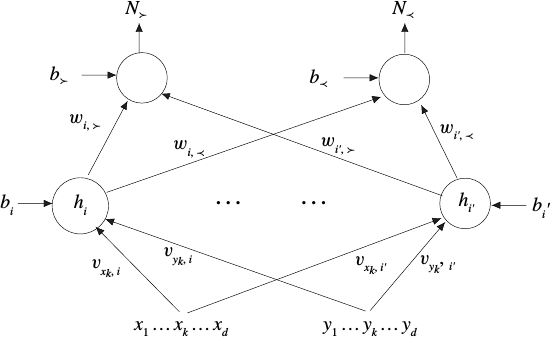
\includegraphics[width=.45\textwidth]{fig1}
\caption{شبکه\ ی معرفی شده\ ی \مق{CmpNN} جهت مقایسه\ ی ارجحیت بین \کادربی{نمونه\ ها}}\label{fig:cmpnn}
\end{figure}
شبکه\ های عصبی در حالت عمومی خواص ۱ و ۲ را نمی\ توانند ارضا کنند لذا در توضیح این روش آمده است که برای این\ که خواص ۱ و ۲ را بتوانند ارضا شوند باید از تکنیک اشتراک گذاری وزن\ ها استفاده شود. با توجه به نماد گذاری مقاله\ ی اصلی $\upsilon_{x_k, i}$($\upsilon_{y_k, i}$) به معنی این است که یال متصل از ورودی $x$ بعد $k$ام به نورون $i$ام لایه\ ی مخفی و $w_{i,\succ}$($w_{i,\prec}$) یال متصل بین نورون $i$ام لایه\ ی مخفی به خروجی $\succ$ شبکه می\ باشند(به شکل \ref{fig:cmpnn} توجه کنید).\بند
برای اشتراک گذاری وزن\ ها هر دو وزن در هر لایه وزن\ هایشان به اشتراک گذاشته می\ شوند. به\ این صورت که برای وزن\ های بین ورودی\ ها و لایه\ ی مخفی
$\upsilon_{x_k, i'} = \upsilon_{y_k, i}$ و  $\upsilon_{y_k, i'} = \upsilon_{x_k, i}$
یعنی وزن\ هایی بین دو نورون از لایه\ ی مخفی و دو عدد از ورودی\ های(دو بعد از دو نمونه\ ی $x$ و $y$) با هم به اشتراک گذاشته می\ شوند؛ همچنین بایاس\ های لایه\ ی مخفی نیز اشتراک وزن دارند و در مورد وزن\ های بین لایه\ ی مخفی و خروجی\ ها به در دو وزن از دو نورون متفاوت از لایه\ ی مخفی به دو خروجی به اشتراک گذاشته می\ شود(همانند کاری که در اشتراک وزن بین ورودی\ ها و لایه\ ی مخفی صورت گرفت).
\زیرقسمت{یادگیری رتبه\ بندی با \مق{SortNet}}
اکنون که با شبکه\ ای که می\ تواند ارحجیت بین داده\ ها را یادبگیرد آشنا شدیم، به معرفی الگوریتم جهت آموزش این شبکه که باعث می\ شود شبکه\ ی \مق{CmpNN} بهترین وزن\ های ممکن متناسب با داده\ های را داشته باشد که در نهایت باعث می\ شود که ارحجیت\ بندی بهتری داشته باشیم. الگوریتمی که در اینجا معرفی می\ شود \مق{SortNet} نام دارد، که مرتبه\ ی اجرایی این الگوریتم $\mathcal{O}(n\log n)$ می\ باشد.\بند
در مورد ضرورت داشتن الگوریتم \مق{SortNet} می\ توان به این نکته اشاره کرد که اگر فرض کنیم به تعداد $N$ عدد نمونه\ ی آزمایشی داشته باشیم، حال اگر رابطه\ ی ارجحیت هر جفت نمونه\ ی موجود در این دیتاست را داشته باشیم به تعداد
$N \choose 2$
عدد رابطه\ ی ارجحیت خواهیم داشت که آموزش این مقدار نیازمند زمان زیادی می\ باشد، لذا نیاز به الگوریتمی داریم که بتواند داده\ های ارجحیت را به صورت هدفمند برای آموزش شبکه\ ی \مق{CmpNN} استفاده کند، که این عمل را الگوریتم \مق{SortNet} انجام می\ دهد که در شکل
\ref{fig:sortnet}
آمده است.
\begin{figure}
\centering
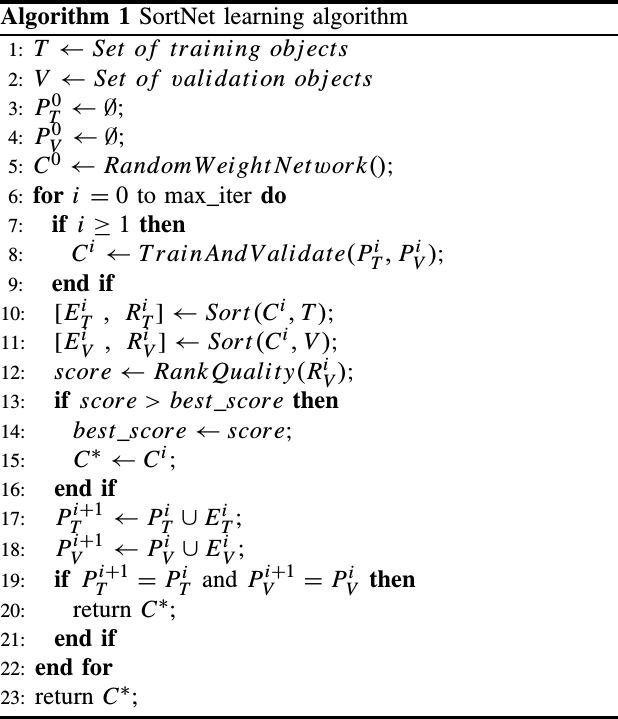
\includegraphics[width=0.45\textwidth]{algorithm1}
\caption{الگوریتم \مق{SortNet}}\label{fig:sortnet}
\end{figure}
در این الگوریتم در هر دوره\زیرنویس{\مق{Iteration}} از آموزش، داده\ های آموزش توسط نمونه\ های جدید گسترش پیدا می\ کند. هدف از این کار این است که زیرمجموعه\ ای آموزشی از داده\ های آموزشی و تست انتخاب شود که دارای حداکثر بهره\ ی اطلاعاتی جهت بروزرسانی وزن\ های شبکه\ ی \مق{CmpNN} باشند. هر مجموعه\ ی آموزشی برای آموزش شبکه\ ی \مق{CmpNN} متفاوتی استفاده می\ شود. فرض کنید تابعی به نام \مق{RankQuality} را داریم که میزان کیفیت یک رتبه\ بندی\زیرنویس{Rank} را ارزیابی می\ کند؛ نتیجه\ ی این الگوریتم تکراری شبکه\ ای است که بهترین نتیجه را بر اساس معیار ارزیابی داشته باشد. در الگوریتم \مق{SortNet} مجموعه\ های
$P_V^i$ و $P_T^i$
شامل جفت نمونه\ هایی ارزیابی و آموزشی هستند که با آن\ ها شبکه\ ی عصبی را آموزش می\ دهیم. در ابتدا این مجموعه\ های تهی هستند
($P_V^0$ و $P_T^0$ -- خطوط ۳ و ۴)
و شبکه به صورت تصادفی وزن\ دهی می\ شوند(خط ۵) و در ابتدا به شبکه\ ی خام(آموزش ندیده) داده\ های آموزشی و تست را می\ دهیم و نمونه\ هایی که توسط شبکه درست و غلط ارجحیت\ بندی شده اند را بدست می\ آوریم(خطوط ۱۰ و ۱۱) سپس برای آن\ هایی در مجموعه\ ی تست درست ارحجیت\ بندی شده\ اند را به تابع ارزیاب کیفیت می\ دهیم و امتیاز ارحجیت\ بندی مجموعه را بدست می\ آوریم(خط ۱۲) و در صورتی که این امتیاز از بهترین امتیاز بدست آمده تاکنون بیشتر باشد امتیاز و شبکه\ ی متناظر با آن را را به عنوان شبکه\ ی برگزیده ذخیره می\ کنیم(خطوط ۱۳ تا ۱۶). سپس داده\ های خطادار از مجموعه\ ی آموزشی و تست به ترتیب به داده\ هایی آموزشی و تستی که در دوره\ ی\زیرنویس{\مق{Iteration}} بعد که می\ خواهیم با آن\ ها شبکه را آموزشی دهیم و ارزیابی کنیم(خطوط ۷ تا ۹) اضافه می\ کنیم(خطوط ۱۷ و ۱۸) و در صورتی که شبکه خطایی نداشته باشد بهترین شبکه\ ی بدست آمده تاکنون را به عنوان خروجی برمی\ گردانیم(خطوط ۱۹ تا ۲۱). در صورتی که به حداکثر تعداد دوره رسیدیم بهترین شبکه\ ی بدست آمده را به عنوان خروجی برمی\ گردانیم(خط ۲۳).
\زیرقسمت{ارزیابی کیفیت رتبه\ بندی}
در این مقاله ۳ تابع ارزیابی کیفیت رتبه\ بندی(\مق{Ranking Quality}) را معرفی کرده است که به شرح زیر می\ باشند:
\begin{enumerate}
\فقره \textbf{\مق{P@n}:} این معیار به صورت میزان ارتباط $n$ مستند\زیرنویس{\مق{Document}} اول که رتبه\ بندی به آن\ ها ارجحیت بالاتری داده است را مشخص می\ کند؛ که به صورت زیر تعریف می\ شود:
\begin{equation}
\text{P@n} = {\text{relevant docs in top n results} \over n}
\end{equation}
\فقره \textbf{\مق{MAP}:} به عنوان میانگین\ گیری بروی معیار \مق{P@n} می\ باشد:
\begin{equation}
\text{AP}_q = {\sum_{n = 1}^{N_q} \text{P@n}\cdot \text{rel}(n) \over N_q}
\end{equation}
که در این\ جا \مق{$N_q$} تعداد مستندات موجود در پرس\ وجو\زیرنویس{\مق{Query}} $q$ می\ باشد. \مق{rel($q$)} در زمانی که $n$امین مستند در مجموعه مرتبط با پرس\ وجو می\ باشد مقدار ۱ را اختیار می\ کند در غیر این صورت ۰ بر می\ گرداند.
\فقره \textbf{\مق{NDCG@n}:} به عنوان یک استخراج کننده\ ی صریح امتیازات رتبه\ ی بندی مجموعه مستندات معرفی شده است:
\begin{equation}
\text{NDCG@n} \equiv Z_n\Bigg((2^{r_1} - 1) + \sum_{j = 2}^n{2^{r_j} - 1 \over \log(j)}\Bigg)
\end{equation}
که در این\ جا
$r_j \geq 0$
میزان ارتباط مستند $j$ام با موضوع مورد پرس\ وجو می\ باشد(برای مستندات با ارتباط ضعیف این مقدار کوچک است) و $Z_n$ یک فاکتور نرمال\ سازی می\ باشد بگونه\ ای که مقدار \مق{NDCG@n} برای مرتب\ سازی ایده\ آل\زیرنویس{\مق{Ideal Ordering}} مقدار ۱ داشته باشد.
\end{enumerate}
\زیرقسمت{آزمایش\ ها}
در آزمایشات از دیتاست\ هایی که توسط آزمایشگاه تحقیقاتی آسیا میکروسافت استفاده شده است که برای رتبه\ بندی و تعیین اولیت مستندات به ازای پرس\ وجوهای مختلف استفاده می\ شوند. در این\ جا از نسخه\ ی ۲.۰ این مجموعه دیتاست استفاده شده است که شامل ۳ دیتاست زیر می\ باشد:
\begin{enumerate}
\فقره \textbf{\مق{TD2003}:} شامل ۵۰ مجموعه\ ی داده متناظر با ۵۰ پرس\ وجو که هریک شامل ۱۰۰۰ مستند می\ باشند. در این دیتاست هر زوج مرتب «پرس\ وجو، مستند» توسط ۴۴ مقدار که معمولا در بازیابی اطلاعات\زیرنویس{\مق{Information Retrieval}} استفاده می\ شوند؛ نمایش داده\ می\ شوند. برچسب\ های تخصیص یافته به هر مستند نشان دهنده\ ی میزان ارتباط(\مق{Relevent (R)}) و عدم\ ارتباط(\مق{Not Relevent (NR)}) می\ باشد. به ازای هر پرس\ وجو فقط ۱٪ از مستندات مرتبط با موضوع آن می\ باشند.
\فقره \textbf{\مق{TD2004}:} همانند \مق{TD2003} می\ باشد با این تفاوت که شامل ۷۵ مجموعه\ ی داده\ ای تفاوت می\ باشد.
\فقره \textbf{\مق{OHSUMED}:} یک دیتاست مرتبط با کاربردهای پزشکی می\ باشد که شامل ۱۰۶ مجموعه\ ی مستندات پزشکی با میزان ارتباط موضوعی به ازای پرس\ وجوهای مختلف می\ باشد. در این دیتاست میزان ارتباط موضوعی هر پرس\ وجو با هر مستند توسط انسان تعیین شده\ اند که توسط ۳ مقدار ارتباط(\مق{R})، عدم\ ارتباط(\مق{NR}) و احتمالا\ مرتبط(\مق{PR}) نشان داده شده\ اند. مستندات توسط ۲۵ ویژگی نمایش داده شده\ اند.
\end{enumerate}
در ابتدای آزمایشات به بررسی و مقایسه\ ی علمکرد شبکه\ ی \مق{CmpNN} با یکی از روش\ های دیگر بروی یادگیری تابع ارجحیت غیرمتعدی می\ پردازیم که در جدول
\ref{tab:1}
آمده است. نتایج میانگینی از نتایج اجرای \مق{5-Fold CrossValidation} می\ باشد که در هر اجرا به\ صورت تصادفی ۱۰,۰۰۰ نمونه جهت آموزش و ۴,۰۰۰ نمونه جهت ارزیابی و ۶,۰۰۰ نمونه جهت تست استفاده شدند. آزمون آماری \مق{t} تایید کرد که مدل ارائه شده در این مقاله بهبود قابل ملاحظه\ ای نسبت به روش دیگر داشته است. در جدول
\ref{tab:3}
نیز عملکرد \مق{CmpNN} با تغییر تعداد نورون\ های لایه\ ی مخفی بروی ۳ دیتاست
\lr{TD2003}, \lr{TD2004} و \lr{OHSUMED}
آورده شده است. در جدول
\ref{tab:4}
نیز تعداد نورون\ های لایه\ ی مخفی برای دیتاست\ ها و توابع ارزیاب کیفیت مختلف آورده شده است که مبنای مقایسه\ های سایر نتایج آزمایشات دیگر این مقاله می\ باشد. در جداول
\ref{tab:5}, \ref{tab:6} و \ref{tab:7}
نتایج اجرای الگوریتم\ های مختلف به ترتیب بروی دیتاست\ های \مق{TD2003}، \مق{TD2004} و \مق{OHSUMED} که با معیارهای \مق{NDCG@n} و \مق{P@n} ارزیابی شده\ اند، نتایج نشان داده\ اند که الگوریتم معرفی شده(\مق{SortNet}) توانسته است در هر ۳ دیتاست مورد آزمون، نتایج بهتری از دیگر الگوریتم\ های مدرن در این زمینه بدست آورد. در جدول
\ref{tab:8}
نیز نتایج اجرای الگوریتم\ های مختلف بروی ۳ دیتاست معرفی شده که با معیار \مق{MAP} سنجیده شده\ اند، آورده شده است، همان\ طور که می\ بینیم الگوریتم معرفی شده با این معیار مقایسه نیز توانسته بهتر از دیگر روش\ های مدرن عمل کند.
\begin{table}
\centering
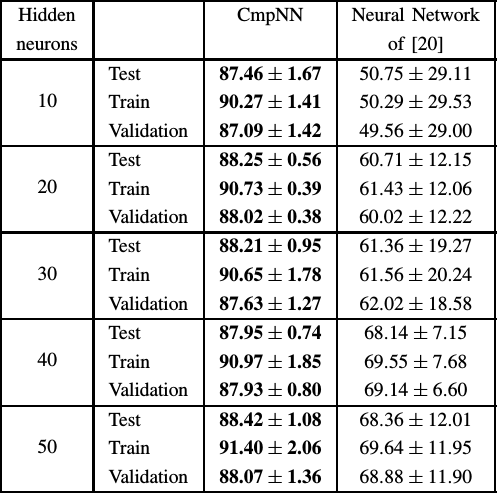
\includegraphics[width=.4\textwidth]{tab1}
\caption{مقایسه\ ی عملکرد شبکه\ ی \مق{CmpNN} با یک روش دیگر برای یادگیری تابع ارجحیت بروی داده\ های غیرمتعدی}\label{tab:1}
\end{table}
\begin{table}
\centering
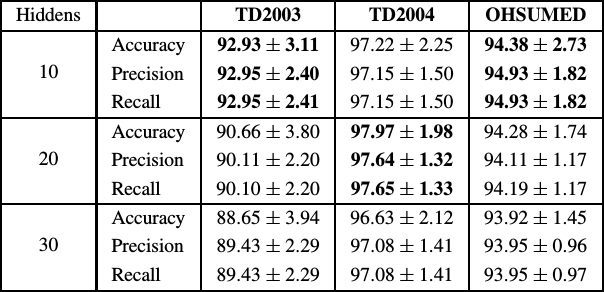
\includegraphics[width=.45\textwidth]{tab3}
\caption{مقایسه\ ی عملکرد شبکه\ ی \مق{CmpNN} با تغییر تعداد نورون\ های لایه\ ی مخفی بروی دیتاست\ های مختلف}\label{tab:3}
\end{table}
\begin{table}
\centering
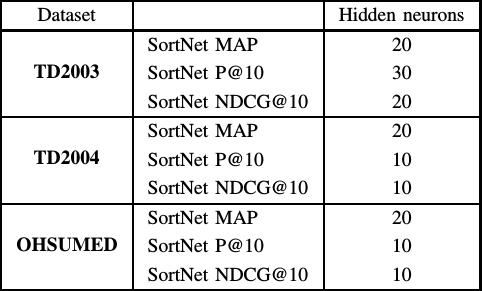
\includegraphics[width=.45\textwidth]{tab4}
\caption{تعداد نورون\ های لایه\ ی مخفی مورد استفاده در شبکه\ ی \مق{CmpNN} در دیتاست\ های مختلف و توابع ارزیاب کیفیت مختلف}\label{tab:4}
\end{table}
\begin{table*}
\centering
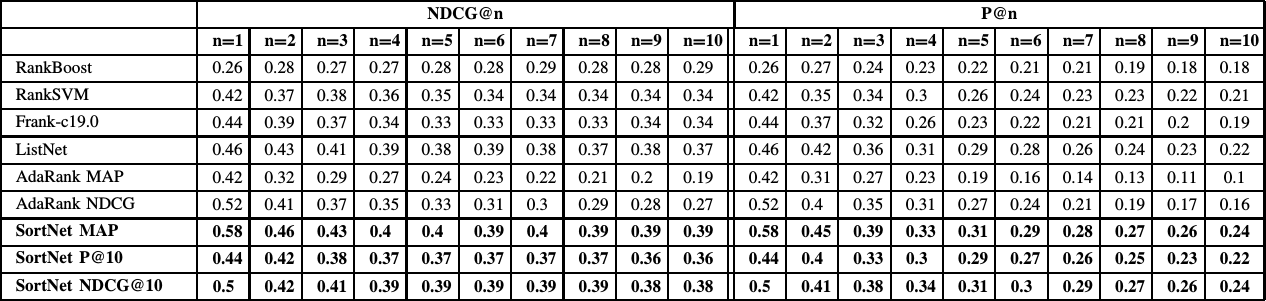
\includegraphics[width=\textwidth]{tab5}
\caption{نتایج اجرای الگوریتم\ های مختلف بروی دیتاست \مق{TD2003} براساس معیارهای \مق{NDCG@n} و \lr{P@n}}\label{tab:5}
\end{table*}
\begin{table*}
\centering
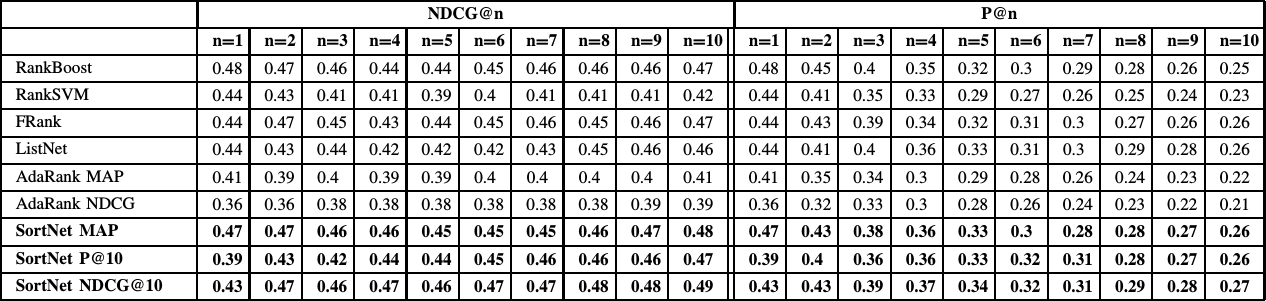
\includegraphics[width=\textwidth]{tab6}
\caption{نتایج اجرای الگوریتم\ های مختلف بروی دیتاست \مق{TD2004} براساس معیارهای \مق{NDCG@n} و \lr{P@n}}\label{tab:6}
\end{table*}
\begin{table*}
\centering
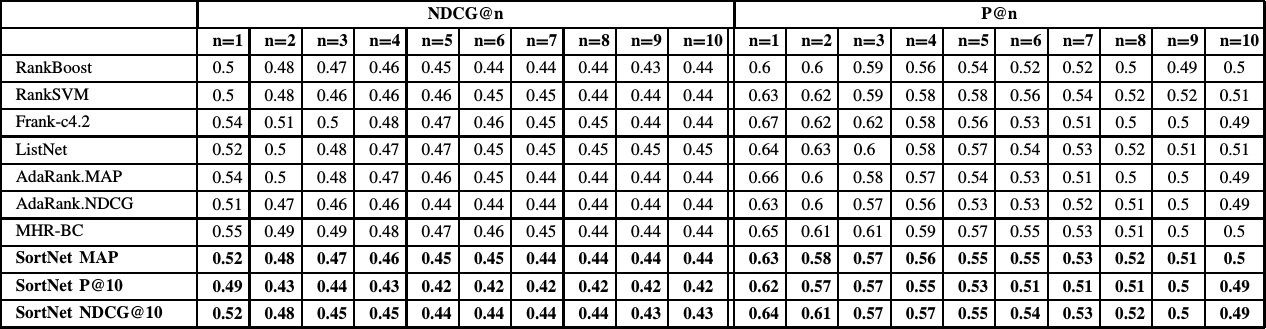
\includegraphics[width=\textwidth]{tab7}
\caption{نتایج اجرای الگوریتم\ های مختلف بروی دیتاست \مق{OHSUMED} براساس معیارهای \مق{NDCG@n} و \lr{P@n}}\label{tab:7}
\end{table*}
\begin{table}
\centering
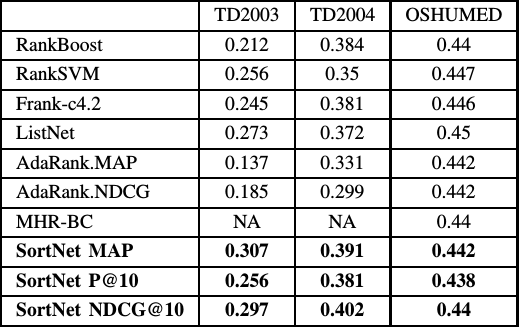
\includegraphics[width=.45\textwidth]{tab8}
\caption{نتایج اجرای الگوریتم\ های مختلف بروی ۳ دیتاست مورد استفاده براساس معیار مقایسه\ ی \lr{MAP}}\label{tab:8}
\end{table}
\newpage
\قسمت{نتیجه\ گیری}
در این گزارش ابتدا به بیان مفاهیم پایه\ ی \یا پرداختیم سپس با مروری خلاصه بر برخی کارهای انجام شده در زمینه\ ی \یا با تمرکز بروی مقاله\ ی اصلی سمینار به معرفی معماری جدیدی از شبکه\ ای عصبی که می\ تواند مدل ارجحیت بین داده\ ها را یادبگیرد پرداختیم سپس الگوریتمی که برای یادگیری بهینه\ ی شبکه استفاده می\ شود را شرح دادیم و در نهایت به ارائه نتایج حاصل از اجرای این شبکه و الگوریتم معرفی شده و مقایسه\ ی این نتایج با اجرای دیگر الگوریتم\ های مدرن در این زمینه پرداختیم و نشان دادیم که روش ارائه شده توانسته است با هر ۳ معیار ارزیابی کیفیت بهتر از دیگر روش عمل کند.
\nocite{*}
\begin{thebibliography}{1}
\begin{latin}\scriptsize

\bibitem{PL:MAIN_1}
Rigutini, L., Papini, T., Maggini, M., Scarselli, F., \emph{"SortNet: Learning to Rank by a Neural Preference Function,"} in Neural Networks, IEEE Transactions on , vol.22, no.9, pp.1368-1380, Sept. 2011

\bibitem{PL:MAIN_2}
Han-Jiang Lai, Yan Pan, Yong Tang, Rong Yu, \emph{"FSMRank: Feature Selection Algorithm for Learning to Rank,"} in Neural Networks and Learning Systems, IEEE Transactions on , vol.24, no.6, pp.940-952, June 2013

\bibitem{PL:MAIN_3}
Fei Gao, Dacheng Tao, Xinbo Gao, Xuelong Li, \emph{"Learning to Rank for Blind Image Quality Assessment,"} in Neural Networks and Learning Systems, IEEE Transactions on , vol.26, no.10, pp.2275-2290, Oct. 2015

\bibitem{PL:PL_PEDIA}
J. Furnkranz and E. Hullermeier, \emph{"Encyclopedia of Machine Learning"}. Springer, 2010, ch. Preference Learning, pp. 789–795.

\bibitem{PL:PL_FRAME}
J. Furnkranz and E. Hullermeier, \emph{"Preference Learning"}. Kunstliche Intelligenz, pp. 60–61, 2005.

\end{latin}
\end{thebibliography}
\newpage
\begin{latin}
\theendnotes
\end{latin}

\end{document}


